% Acciones y transiciones de estado del modelo con giro (GridRobot).
% Cada panel parte del mismo estado, con el robot orientado hacia la derecha.
\providecommand{\ejeH}{c}
\providecommand{\ejeV}{r}
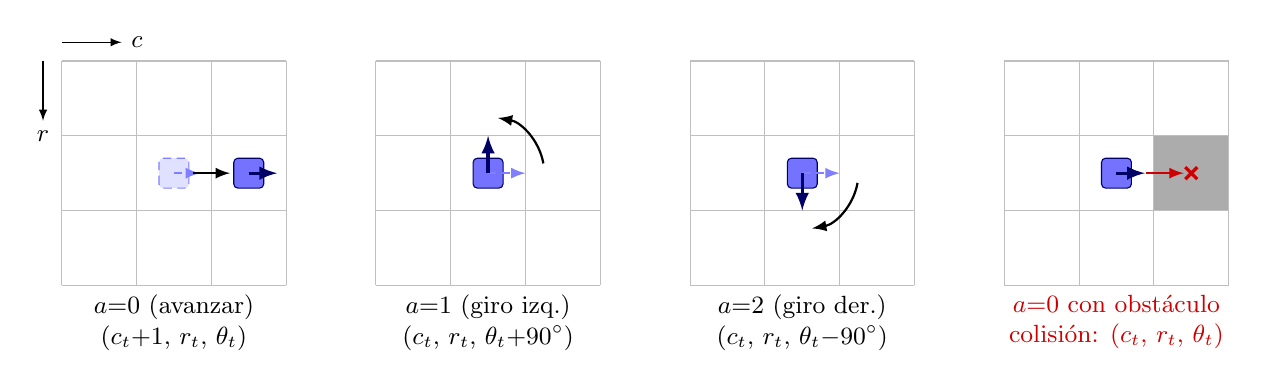
\begin{tikzpicture}[scale=0.95, >=latex,
        robot/.style={fill=blue!55, draw=blue!40!black, rounded corners=1.5pt},
        previo/.style={fill=blue!12, draw=blue!50, densely dashed, rounded corners=1.5pt},
        rumbo/.style={->, very thick, blue!40!black},
        rumboprevio/.style={->, thick, blue!50, densely dashed},
        accion/.style={font=\small, align=center}]
    % Ejes de la rejilla (origen arriba a la izquierda), comunes a los paneles
    \draw[->] (0,3.25) -- (0.8,3.25) node[right] {\small $\ejeH$};
    \draw[->] (-0.25,3) -- (-0.25,2.2) node[below] {\small $\ejeV$};
    % a = 0: avanzar
    \begin{scope}
        \draw[gray!50] (0,0) grid (3,3);
        \draw[previo] (1.3,1.3) rectangle (1.7,1.7);
        \draw[rumboprevio] (1.5,1.5) -- (1.85,1.5);
        \draw[->, thick] (1.75,1.5) -- (2.25,1.5);
        \draw[robot] (2.3,1.3) rectangle (2.7,1.7);
        \draw[rumbo] (2.5,1.5) -- (2.88,1.5);
        \node[accion, below] at (1.5,0)
            {$a{=}0$ (avanzar)\\ $(\ejeH_t{+}1,\,\ejeV_t,\,\theta_t)$};
    \end{scope}
    % a = 1: giro a la izquierda
    \begin{scope}[shift={(4.2,0)}]
        \draw[gray!50] (0,0) grid (3,3);
        \draw[robot] (1.3,1.3) rectangle (1.7,1.7);
        \draw[rumboprevio] (1.5,1.5) -- (2.0,1.5);
        \draw[rumbo] (1.5,1.5) -- (1.5,2.0);
        \draw[->, thick] (1.5,1.5) ++(10:0.75) arc (10:80:0.75);
        \node[accion, below] at (1.5,0)
            {$a{=}1$ (giro izq.)\\ $(\ejeH_t,\,\ejeV_t,\,\theta_t{+}90^\circ)$};
    \end{scope}
    % a = 2: giro a la derecha
    \begin{scope}[shift={(8.4,0)}]
        \draw[gray!50] (0,0) grid (3,3);
        \draw[robot] (1.3,1.3) rectangle (1.7,1.7);
        \draw[rumboprevio] (1.5,1.5) -- (2.0,1.5);
        \draw[rumbo] (1.5,1.5) -- (1.5,1.0);
        \draw[->, thick] (1.5,1.5) ++(-10:0.75) arc (-10:-80:0.75);
        \node[accion, below] at (1.5,0)
            {$a{=}2$ (giro der.)\\ $(\ejeH_t,\,\ejeV_t,\,\theta_t{-}90^\circ)$};
    \end{scope}
    % a = 0 con la celda frontal ocupada
    \begin{scope}[shift={(12.6,0)}]
        \fill[gray!65] (2,1) rectangle (3,2);
        \draw[gray!50] (0,0) grid (3,3);
        \draw[robot] (1.3,1.3) rectangle (1.7,1.7);
        \draw[rumbo] (1.5,1.5) -- (1.88,1.5);
        \draw[->, thick, red!80!black] (1.9,1.5) -- (2.4,1.5);
        \draw[red!80!black, very thick] (2.42,1.42) -- (2.58,1.58)
            (2.42,1.58) -- (2.58,1.42);
        \node[accion, below, text=red!80!black] at (1.5,0)
            {$a{=}0$ con obstáculo\\ colisión: $(\ejeH_t,\,\ejeV_t,\,\theta_t)$};
    \end{scope}
\end{tikzpicture}
